\documentclass[a4paper]{article}

%% Language and font encodings
\usepackage[english]{babel}
\usepackage[utf8x]{inputenc}
% \usepackage[garamond]{mathdesign}
\usepackage[math]{blindtext}
\usepackage[T1]{fontenc}
\usepackage{mathptmx}
\usepackage[12pt]{moresize}
%% \usepackage{ebgaramond,newtxmath,ebgaramond-maths}

%% Sets page size and margins
\usepackage[a4paper,top=1in,bottom=1in,left=1in,right=1in,marginparwidth=1.75cm]{geometry}

\usepackage{setspace}
\onehalfspacing


%% Useful packages
\usepackage{amsmath}
\usepackage{graphicx}
\usepackage[colorinlistoftodos]{todonotes}
\usepackage[colorlinks=true, allcolors=blue]{hyperref}
\usepackage{natbib}
\setlength{\bibsep}{0pt plus 0.3ex}
\usepackage{algorithm}
\usepackage{tikz}
\usepackage[noend]{algpseudocode}
\usepackage{float}
\usepackage{listings}
\usepackage{color}
 
\definecolor{codegreen}{rgb}{0,0.6,0}
\definecolor{codegray}{rgb}{0.5,0.5,0.5}
\definecolor{codepurple}{rgb}{0.58,0,0.82}
\definecolor{backcolour}{rgb}{0.95,0.95,0.92}
 
\lstdefinestyle{mystyle}{
    backgroundcolor=\color{backcolour},   
    commentstyle=\color{codegreen},
    keywordstyle=\color{magenta},
    numberstyle=\tiny\color{codegray},
    stringstyle=\color{codepurple},
    basicstyle=\footnotesize,
    breakatwhitespace=false,         
    breaklines=true,                 
    captionpos=b,                    
    keepspaces=true,                 
    numbers=left,                    
    numbersep=5pt,                  
    showspaces=false,                
    showstringspaces=false,
    showtabs=false,                  
    tabsize=2
}
 
\lstset{style=mystyle}

\newcommand{\norm}[1]{\left\lVert#1\right\rVert}

\title{Language Model with LSTM in TensorFlow}
\author{Keping Wang}

\begin{document}
\maketitle

\section{Introduction}
The goal of this paper is to train a word level language model using LSTM (Long Short Term Memory) network and use it to generate text.

A language model is a probability distribution over sequences of words. A language model is trained on a corpus of text, then given a piece of test text, the model will be able to predict the probability that the test text belongs to the this certain language that the model is trained on. Language model is a basic tool in natural language processing, and can be used in tasks like speech recognition, machine translation, part-of-speech tagging etc.

Unsupervised text generation is the ultimate goal in my mind when I'm choosing the topic. It is an understudied field (compared to the recently popular image generation), and I want to make some exploration. I'll have a review about the recent progress in unsupervised text generation in a later section. However, because of limited time and computing power, I'll only try text generation with an LSTM language model. A tuned language model is given a piece of text as input, and will output the following text that it deems most sensible.

\section{Network Model}
The basic network structure of the language model goes as follows: 1) A sequence of words goes into an embedding layer and goes out as a sequence of embedded vectors. 2) A recurrent network of LSTM cells takes the embedded vectors and outputs a sequence of vectors, each of which represents the log probability of each word at that location. 3) The log probability vectors are then used to calculate loss or predict words. I'll explain these three parts in the following three sections.

\subsection{Word Embedding}
One thing that distinguishes word level language processing from other machine learning tasks is that the data is very sparse over the feature space. 

In machine learning we deal with numbers and we have to convert everything into numbers. A direct way to transform words into numbers is to encode a word into a one-hot vector, which has the same dimension as the size of the vocabulary, and the value in the "word-itself" dimension is one, and all other values are zero. For example, if the vocabulary is $[ \text{"hello", "world", "morning"} ]$, then the word "world" will be encoded as $[0, 1, 0]$.

However, one-hot encoding will give us a huge feature space, sparse input data, and lots of parameters, which makes the model hard to train. Actually, we can preserve much of the information in the data while greatly reducing the dimensionality of our data. This is done with word embedding. Word embedding means representing each word with a low dimension vector while retaining much of the information contained in the word. Word embedding itself is a useful tool in natural language processing. Words represented as low dimension vectors will help with lots of tasks down the pipeline. 

A recently popular embedding method is called word2vec \citep{mikolov2013efficient}, which models embeddings as a one hidden layer neural network, takes input of the history before current word, and is trained by minimizing the negative noise-contrastive softmax loss, which approximates the negative probability of the correct word being predicted.\footnote{This version of word2vec is called CBOW. Another version, skip-gram, is to take a single word, and predict its surrounding words within a window.} Google actually has a pretrained word2vec embedding\footnote{\url{https://code.google.com/archive/p/word2vec/}}, which is trained trained on roughly 100 billion words from a Google News dataset, and embeds a 3 million words vocabulary into vectors with 300 features. 

Some good heuristics for understanding the information preserved in embeddings are distance and vector addition/subtraction. Semantically and syntactically\footnote{Some embedding models will be better at semantical similarity, while some better at syntactical similarity.} similar words will be close to each other in the feature space. Also, an example of vector addition/subtraction is that: $v_{king} - v_{queen} \approx v_{man} - v_{woman}$.

The information contained in the embeddings is closely related to the training data and the model used for training, so for specific tasks it might be better to have specifically trained embeddings. In this paper I will train the word embeddings myself. 

Although I've said all the fancy stuff about word embedding, it is really just one extra layer at the beginning of the neural network. It's a little bit special because it is not an affine transformation (like $f_j(x) = w\cdot x+b_j$), not an element-wise activation (like $relu(x)$), but an indexing operation:
\begin{equation}
  v_i = embeddings[x_i], \quad \text{for observation $i$,}
\end{equation}
where $v_i$ is the output embedded vector, $embeddings$ is a large 2d matrix of dimension $vector\_size \times vocabulary\_size$, and $x_i$ is the integer representation of an input word. With embeddings, we can make index accesses with integer index values, without the explicit usage of one-hot word encodings. Then we just do whatever we want with the input vectors $v$ just like in any neural network.

Note that at the end of the network, we usually want to convert our vectors back to words, and that's when we still need the one-hot encodings (in some sense). Here in my language model, the output of the network for a word input will be a vector of dimension $vocabulary\_size$, where each dimension represents the predicted log probability of the corresponding word showing up at that location. Then this output vector will be used to calculate loss and perplexity, the evaluation metric, which I'll introduce in detail later, or be used to pick the max-probability word as the predicted word.

\subsection{LSTM}
I'll briefly explain about recurrent neural networks and LSTM here, but please refer to \cite{colahLSTM} \url{http://colah.github.io/posts/2015-08-Understanding-LSTMs/} for a probably better explanation.

Recurrent neural network is a type of network structure that contains internal states other than just taking input and generating output. Of course every network layer contains weights. But for a sequence of inputs, the states in recurrent networks are changed each time one input of input is feed into the network. 

Instead of one cell processing inputs sequentially, we can also view this as a sequence of weight-sharing cells processing sequential input. Each cell takes a tuple $(input\_data, input\_state)$ as input, and outputs a tuple $(output\_data, output\_state).$\footnote{This mostly comes from the TensorFlow notation. \url{https://www.tensorflow.org/versions/r1.0/api_docs/python/tf/contrib/rnn/RNNCell}} The $output\_state$ from a previous cell will be given as $input\_state$ to the next cell, and note that the previous cell and the next cell are actually the same cell (they share weights). Usually only $output\_data$ is interested for further steps of data processing, and the initial $input\_state$ can be set as all zero. It is perhaps easier to understand in pseudo-code:

\begin{lstlisting}[language=Python]
cell = RNNCell() # construct a new RNN cell instance
initial_state = all_zero_state()
state = initial_state
output1, state = cell.process(input1, state)
output2, state = cell.process(input2, state)
output3, state = cell.process(input3, state)
...
\end{lstlisting}

If we view this whole thing together, it takes an initial state, a sequence of inputs $[input1, input2, input3]$, and generate a sequence of outputs $[output1, output2, output3]$.

LSTM\citep{hochreiter1997long} is a special type of "RNNCell". There are some (a little bit) complex operations in the "process" step, but LSTM is special in that it contains trainable weights that allows the cell to optionally forget previous state. There are variants of LSTM, like GRU \citep{chung2014empirical}, that allow similar functionalities with different implementation in the "process" step. Their performance don't differ much empirically.

Multiple RNN cells can be stacked together to make a deeper recurrent neural network:
\begin{lstlisting}[language=Python]
cell1 = RNNCell()
cell2 = RNNCell()
state1 = all_zero_state()
state2 = all_zero_state()
hidden1, state1 = cell1.process(input1, state1)
output1, state2 = cell2.process(hidden1, state2)
hidden2, state1 = cell1.process(input2, state1)
output2, state2 = cell2.process(hidden2, state2)
hidden3, state1 = cell1.process(input3, state1)
output3, state2 = cell2.process(hidden3, state2)
...
\end{lstlisting}
here "cell1" and "cell2" are stacked as two layers by linking the $output\_data$ of "cell1" and the $input\_data$ of "cell2". 

Currently an RNN cell takes (input, state) and outputs (output, state). Sequential calls of the same cell are linked by "state", and different cells are linked by "input" and "output". RNN is made deeper by simply stacking layers together. This is the specific structure of a recurrent neural network, but could also be viewed as a special case of a general neural network. And it is probably not the only possible way to structure a recurrent neural network. Recently people have discovered innovative ways to structure a deep convolutional neural network, like ResNet \citep{he2016deep} and DenseNet \citep{huang2016densely}, so I believe better structures for recurrent neural networks are also out there for people to discover. Of course, the ideal case would be having a super Meta-learning model that automatically learns different kinds of structures.

In this paper, I use a multi-layer recurrent network with LSTM cells.

\subsection{Dropout}
Dropout is a very simple and extremely useful technique to prevent overfitting of a neural network. Long time ago it is only applied to convolutional networks, then \cite{zaremba2014recurrent} discovered the correct way to implement dropout in RNN. The key point is to only apply dropout to the non-recurrent part of the network, like in the following graph\footnote{Taken from \cite{zaremba2014recurrent}}. 

\begin{figure}[H]
\centering
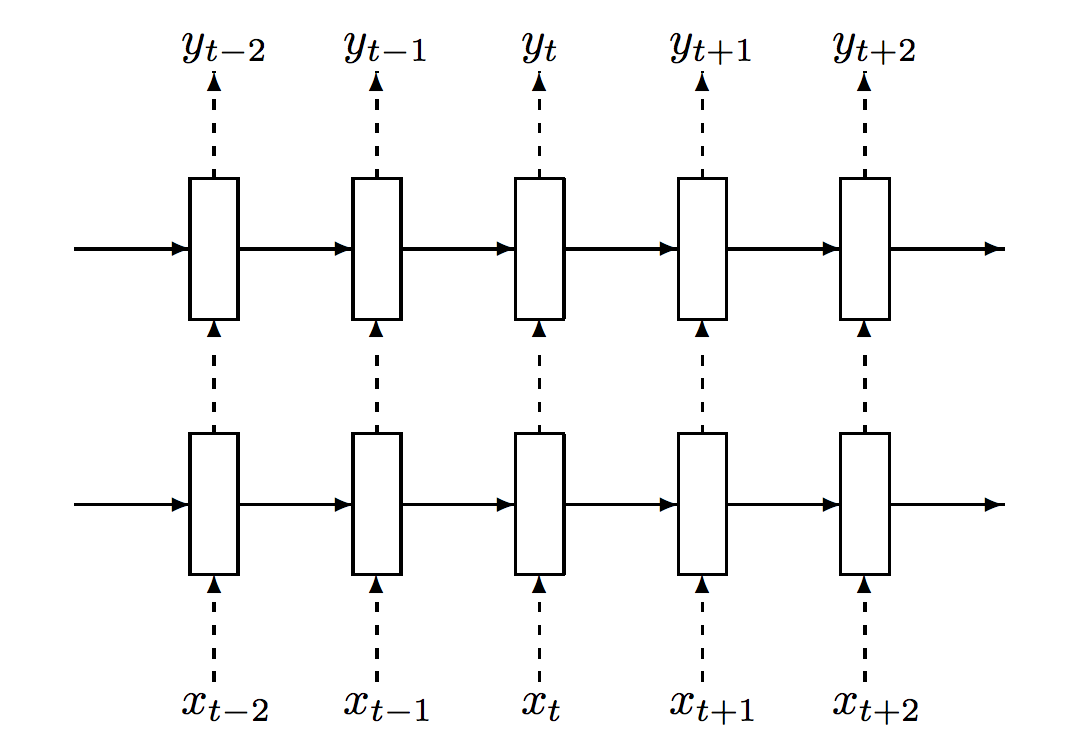
\includegraphics[width=0.6\textwidth]{rnn_dropout.png}
\caption{Dropout in RNN.  The dashed arrows indicate connections where dropout is applied, and the solid lines indicate connections where dropout is not applied.}
\end{figure}

\subsection{Loss and Perplexity}
The loss function I'm using is the softmax cross entropy loss. Let's consider one word $x$. Denote the final output vector as $z := model.process(x)$. $z$ is a vector of dimension $vocabulary\_size$, denoted as $V$. The softmax of $z$ is defined as:
\begin{equation}
  softmax(z) = \frac{[\exp(z_1), ... , \exp(z_V)]}{\sum_{v=1}^V exp(z_v)}.
\end{equation} 

Cross-entropy \citep{karpathy231n} is an information theory concept used to measure the difference between a true distribution $p$ and an estimated distribution $q$:
\begin{equation}
 H(p, q) = - \sum_x p(x) \log q(x)
\end{equation}

And finally the softmax cross-entropy loss is defined as:
\begin{align}
  & loss = - \log \left( \frac{\exp(z_{correct\_word})}{\sum_{v=1}^V exp(z_v)} \right) \\
  & \text{where the estimated distribution } q = \frac{\exp(z_{correct\_word})}{\sum_{v=1}^V exp(z_v)} \\
  & \text{and the "true" distribution } p = [0, ..., 1, ..., 0], \\
  & \quad \quad \text{ where the single one is at the position of the correct word.}
\end{align}

Thus the $\frac{\exp(z_{correct\_word})}{\sum_{v=1}^V exp(z_v)}$ can be interpreted as the normalized probability assigned to the correct word by the model. Vector $z$ can be seen as the unnormalized log probabilities for all words. 

For multiple words per observation, and multiple observations, the total loss is just the mean of losses of all words. 

In language models, we use a metric called Perplexity to evaluate the entropy of a given paragraph with $T$ words:
\begin{align}
  perplexity(w_1, \dots, w_T) & = P(w_1, \dots, w_T)^{-\frac{1}{T}} \\
  & = \prod_{i=1}^T P(w_t|w_1, \dots, w_{t-1}) ^{-\frac{1}{T}}
\end{align}

For a simple metric to report, people usually use average per-word perplexity (often just called perplexity):
\begin{equation}
 \text{average per-word perplexity} = e^{loss}
\end{equation}

\section{Experiments}
I implemented the neural network language model in TensorFlow \citep{tensorflow2015-whitepaper}. The model is trained on novels from Project Gutenberg\footnote{\url{https://www.gutenberg.org/}}. I first run a tiny model on my local machine, and then run a larger model on an AWS p2 instance.

\subsection{Data and Preprocessing}
The data used here are novels from Project Gutenberg, more specifically, 10 novels by Charles Dickens. The following preprocessing is applied to the data: 1) clean up unnecessary new lines, 2) use lowercase for all letters (since it's a word level language model, I don't want it to worry too much about letters), 3) replace all digits with "\#", 4) add spaces around punctuations like ",", ".", ":", etc. 5) split the text by space into a list of words.

\subsection{Results}

First I fit my model over a very small data set with only 2000 words for the training data and 400 words for the test data. The hidden vector is of size 128, and two layers are stacked together. Sequence length is 20.

\begin{figure}[H]
\centering
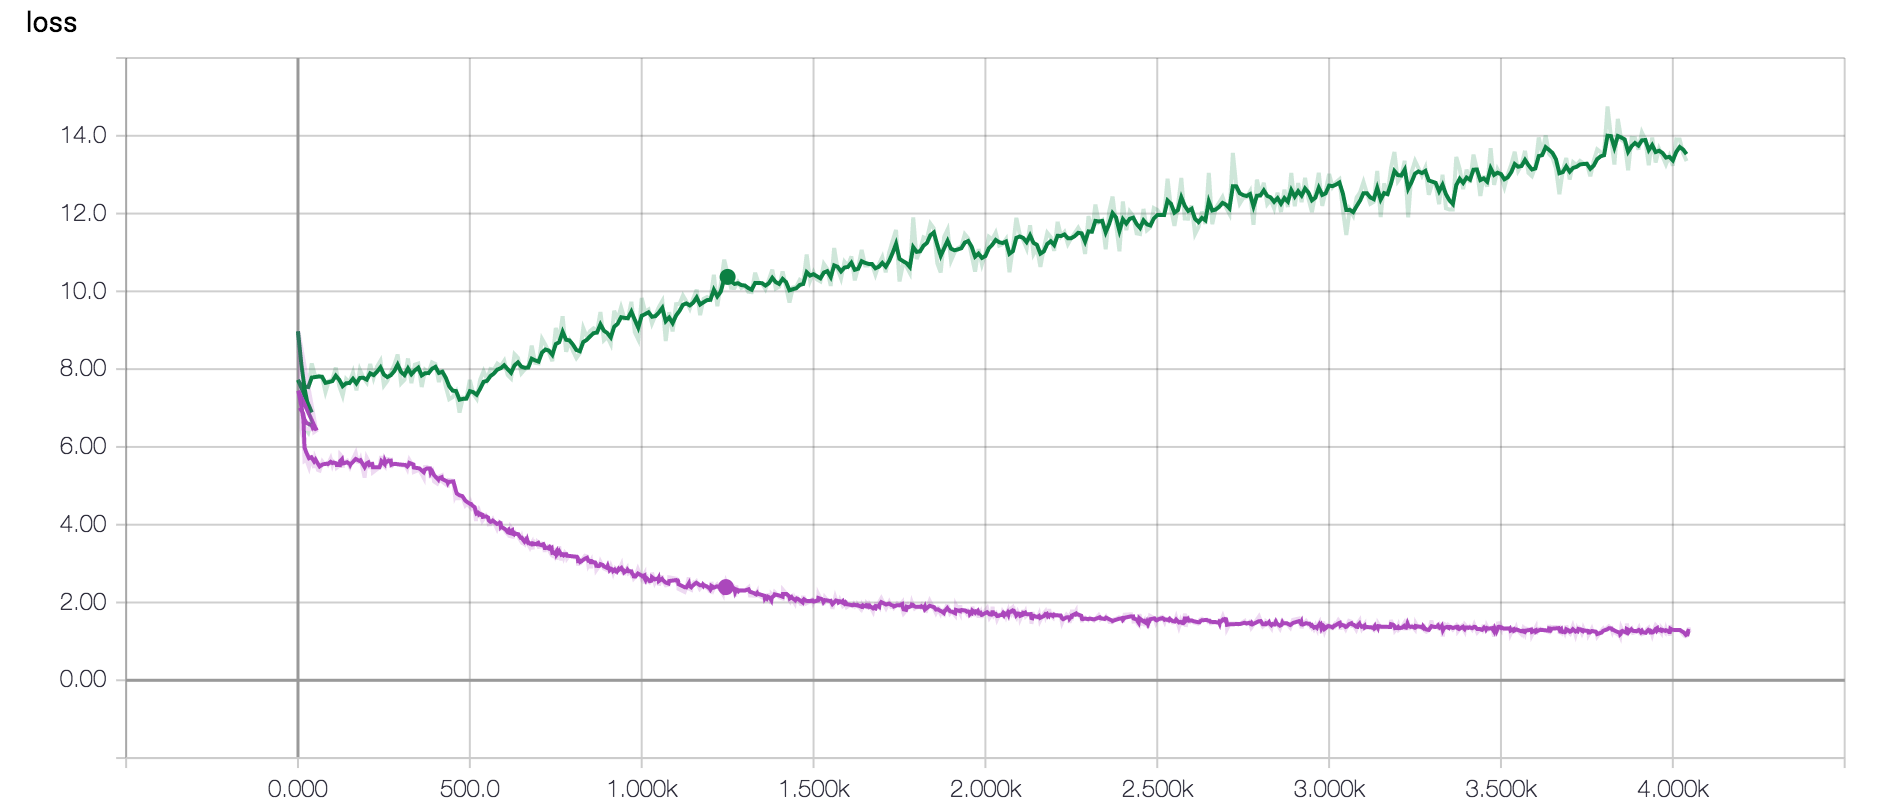
\includegraphics[width=0.8\textwidth]{small_loss.png}
\caption{Loss of a very small data set. Purple for training data, green for test data.}
\end{figure}

\begin{figure}[H]
\centering
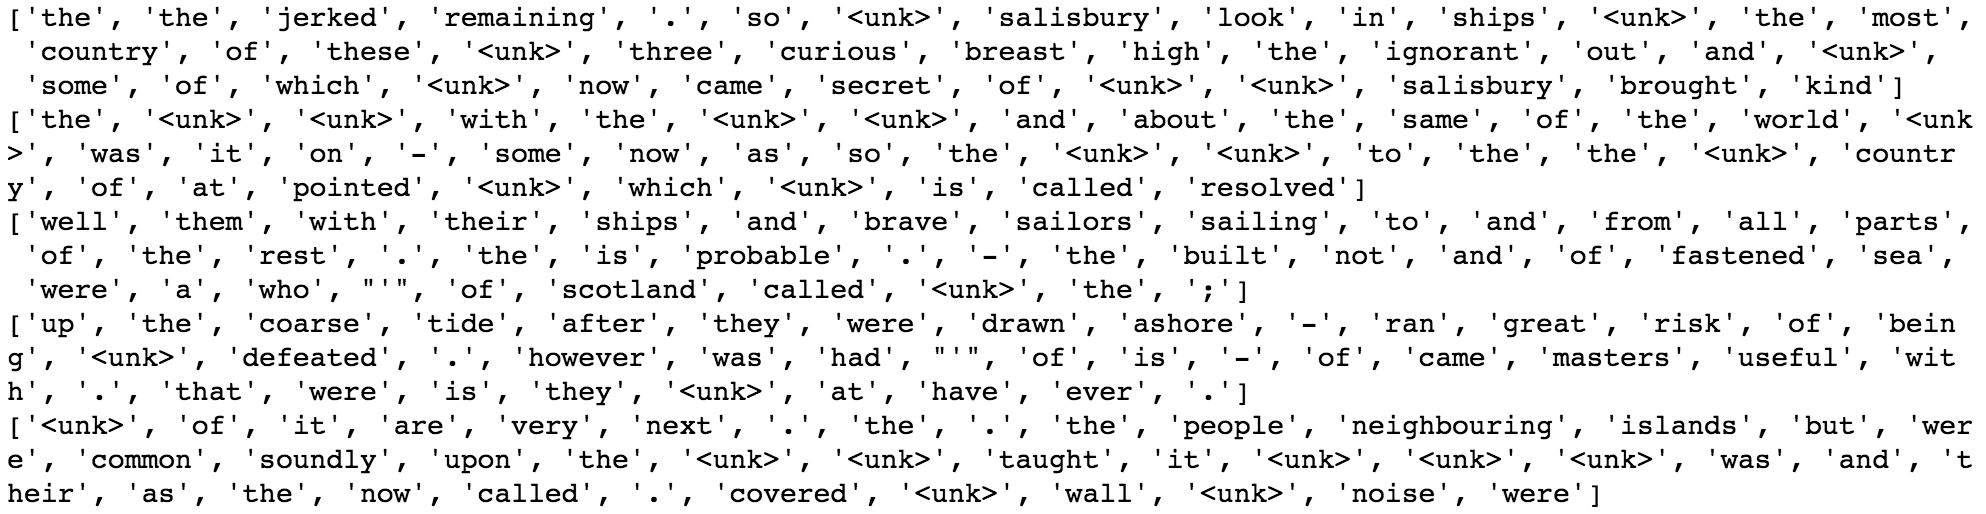
\includegraphics[width=0.8\textwidth]{small_prediction.png}
\caption{Words prediction of a very small model on training data.}
\end{figure}

The language model does overfit the data, and outputs a seemingly a little bit reasonable text. The sequence length is 20, and the first twenty words prediction get input from training data. The next twenty words prediction get inputs from previous outputs. The final training perplexity is about 4. This very small model can be trained with my Macbook Pro CPU in 3 minutes. 

Then I try to fit a large dataset with 2000000 words in training data and 400000 words in test data. It has hidden vector of size 512, and 2 layers. The vocabulary size is capped at 8000, and rare words are denoted as "<unk>". Sequence length is 35. The model file is 264 MB. I run it on an AWS p2 instance for 4 hours but it hasn't been fully trained. That's probably because my learning and its rate decay rate are not properly set. But I don't have the time to fine tune the model. The not-fully-trained results are the follows. The final perplexity score is only about 230.

\begin{figure}[H]
\centering
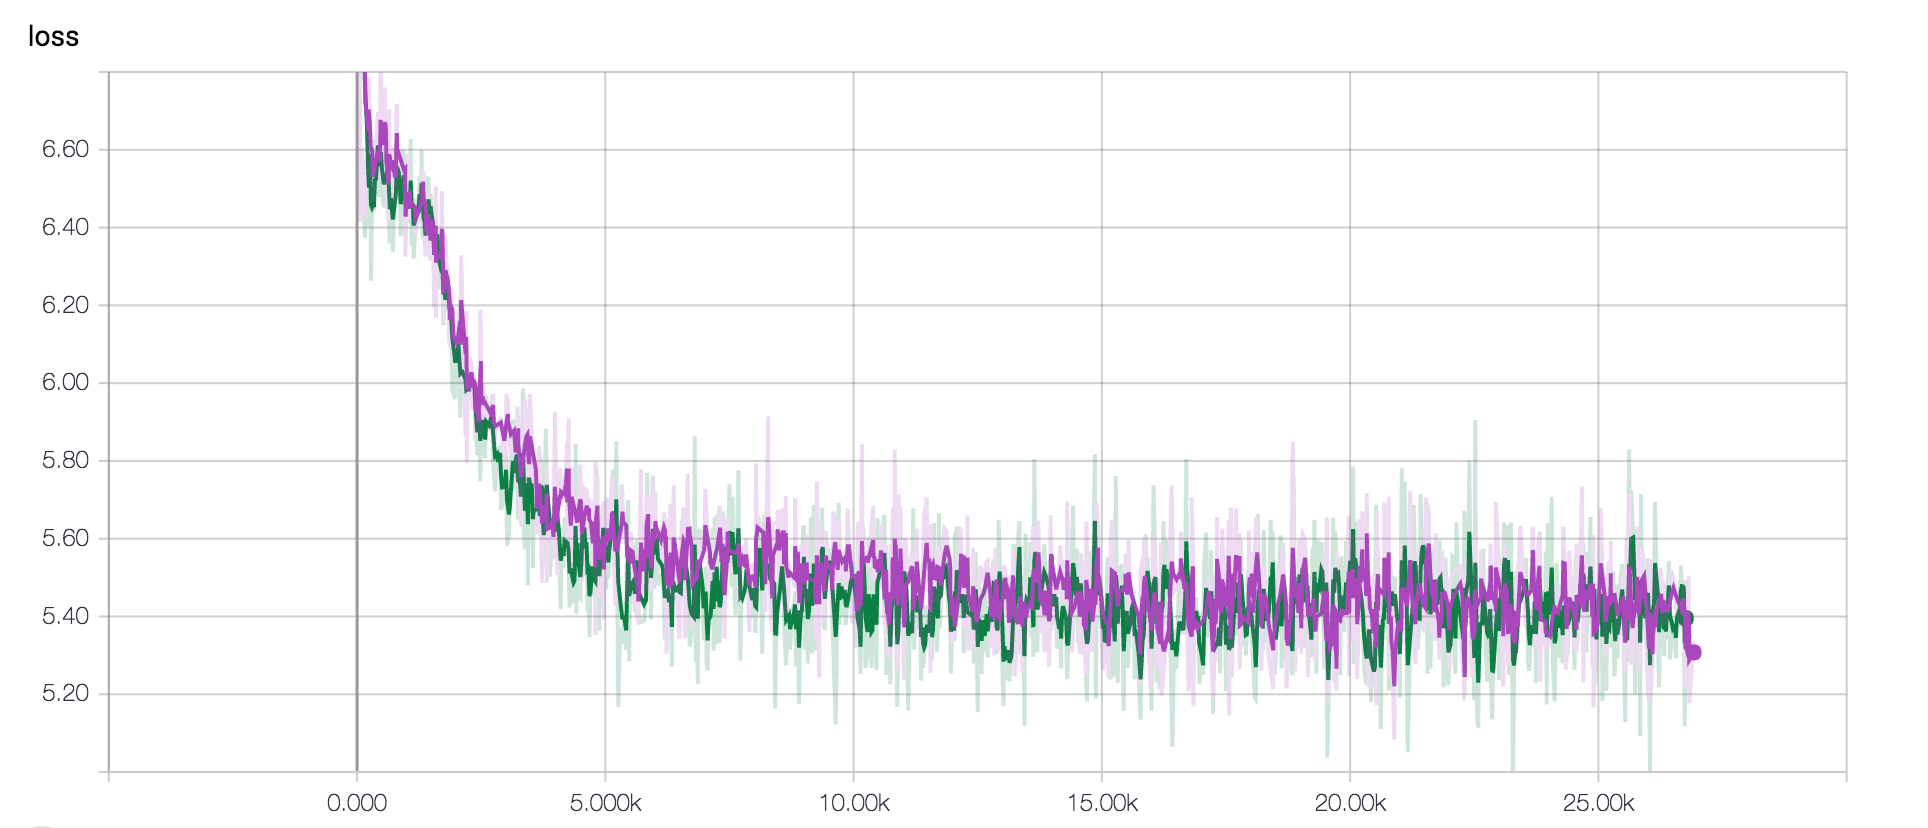
\includegraphics[width=0.8\textwidth]{large_loss.png}
\caption{Loss of a large model, not fully trained}
\end{figure}

\begin{figure}[H]
\centering
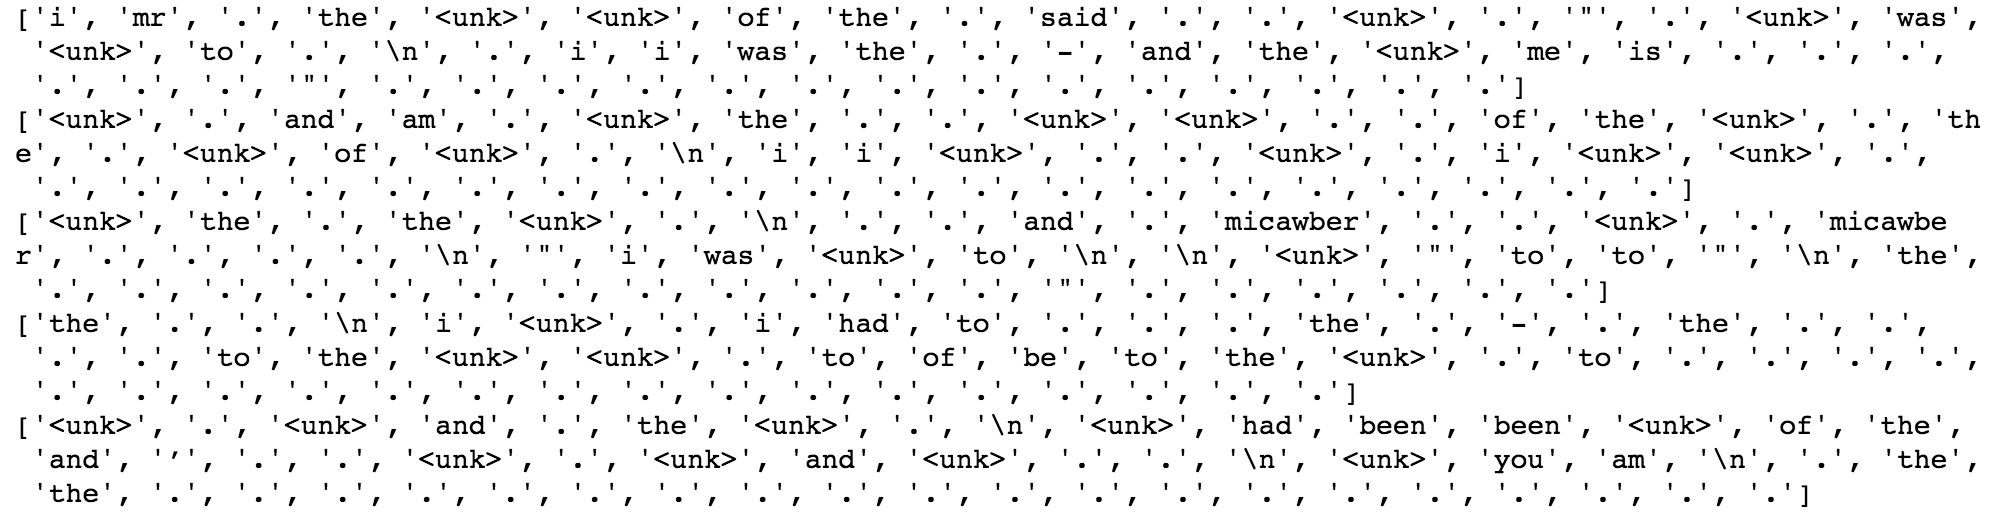
\includegraphics[width=0.8\textwidth]{large_prediction.png}
\caption{Words prediction of the not fully trained large model}
\end{figure}

\section{Analysis}
One pretty good perplexity score of language model on Penn Tree Bank is 78 \citep{zaremba2014recurrent}. While the language model here uses a different dataset since is not directly comparable, the size of Penn Tree Bank and my Dickens novels are somewhat similar. My perplexity score of 230 seems problematic. The model is not fully trained.

When compared with the good character-level RNN\footnote{\url{http://karpathy.github.io/2015/05/21/rnn-effectiveness/}}, the word-level RNN is significantly larger and harder to train. I cannot really well tune the model because it takes so long to train. More experiments should be made to tune the model.

Also for data preprocessing, I only cleaned up some punctuations and newlines, but don't really find the starting point of training texts. The data fed may start from the middle of a sentence. This could be pretty problematic for the RNN since it will be forced to fit a word with incomplete history, and thus gets confused. In the future I would experiment more like feeding data starting at sentence or paragraph beginnings.

\section{Related Work and Future Work}
Although I'm interested in text generation, here in this paper I only tried the simples possible technique for text generation. Overall automatic text generation is an understudied field, but recently people have made some progress.

\cite{textGAN} used a Generative Adversarial Network (GAN) for text generation. Specifically they use an RNN as the generator but a Convolutional Neural Network (CNN) as the discriminator. The CNN technique they use comes from \cite{kim2014convolutional}, where an CNN is applied on top of pre-trained or task-specific word vectors and shows good performance for sentence classification tasks. Differently, \cite{johnson2014effective} applied CNN directly to the high-dimensional text data, which leads to directly learning embeddings of small text regions. Considering the amazing result of GAN on image generation \citep{goodfellow2014generative}, and the effectiveness of CNN for discriminative NLP tasks, we have reasons to believe that text generation with CNN and GAN might be a nice direction to progress.

A different approach is proposed in \cite{yu2016sequence}, which still utilizes GAN, but changes the generative network from RNN with word embedding to an Markov decision process in Reinforcement learning, and then the generator is trained with policy gradient. 

Another effort for text generation is made in \cite{hu2017controllable}. They proposed a neural generative model which combines variational auto-encoder \citep{kingma2013auto} and holistic attribute discriminators for effective imposition of semantic structures. 

So there are lots of possible network structures that could lead to better text generation. In the future I'll try to adopt a GAN for text generation.

\bibliographystyle{alpha}
\bibliography{net}

\end{document}